\documentclass[tikz,border=4pt]{standalone}
% Shared visual grammar: role fills, dark connectors, and 7-point typography.
% Build each standalone figure from this directory. No external images required.
\pdfinfoomitdate=1
\pdftrailerid{}
\usepackage[T1]{fontenc}
\usepackage{helvet}
\renewcommand{\familydefault}{\sfdefault}
\usepackage{amsmath,amssymb}
\hyphenpenalty=10000
\exhyphenpenalty=10000
\usetikzlibrary{arrows.meta,calc,fit,positioning,decorations.pathreplacing,backgrounds}
\definecolor{ink}{HTML}{172B3A}
\definecolor{muted}{HTML}{586D85}
\definecolor{datafill}{HTML}{F1F5F9}
\definecolor{dataline}{HTML}{62748E}
\definecolor{modelfill}{HTML}{E5E9FF}
\definecolor{modelline}{HTML}{7887C7}
\definecolor{llmfill}{HTML}{FFE4E8}
\definecolor{llmline}{HTML}{E68494}
\definecolor{truthfill}{HTML}{D0FAE5}
\definecolor{truthline}{HTML}{35A782}
\newcommand{\seven}{\fontsize{7}{8.5}\selectfont}
\tikzset{
 every node/.append style={font=\seven,text=ink,align=center},
 box/.style={draw=dataline,fill=white,rounded corners=3pt,line width=.65pt,inner sep=5pt,minimum height=8mm},
 data/.style={box,fill=datafill},
 model/.style={box,draw=modelline,fill=modelfill},
 llm/.style={box,draw=llmline,fill=llmfill},
 truth/.style={box,draw=truthline,fill=truthfill},
 title/.style={font=\seven\bfseries,inner sep=1pt},
 word/.style={text=muted,inner sep=1pt,align=center},
 label/.style={fill=white,inner xsep=2pt,inner ysep=1pt,text=muted},
 flow/.style={-{Stealth[length=2.4mm,width=1.9mm]},draw=ink,line width=1.2pt,shorten >=1.5pt},
 branch/.style={-{Stealth[length=2mm,width=1.6mm]},draw=ink,line width=.9pt,shorten >=1pt},
 route/.style={draw=ink,line width=1.2pt},
 update/.style={-{Stealth[length=2.2mm,width=1.7mm]},draw=modelline,line width=1pt,dash pattern=on 3pt off 2pt,shorten >=1.5pt},
 boundary/.style={draw=dataline,dash pattern=on 3pt off 2pt,rounded corners=3pt,line width=.6pt},
 chip/.style={minimum height=4mm,inner xsep=3pt,inner ysep=1.5pt,rounded corners=2pt},
}
% Optional role key. Anchor at the center of an uncluttered final row.
\newcommand{\rolekey}[2]{
 \node[word,anchor=east] at (#1-6.6,#2) {\textit{Key}};
 \node[data,chip] at (#1-5.2,#2) {records / data};
 \node[model,chip] at (#1-1.9,#2) {learned model / policy};
 \node[llm,chip] at (#1+1.65,#2) {LLM signal};
 \node[truth,chip] at (#1+4.95,#2) {labels / evaluation};
}

\definecolor{errorink}{HTML}{B3213D}
\begin{document}
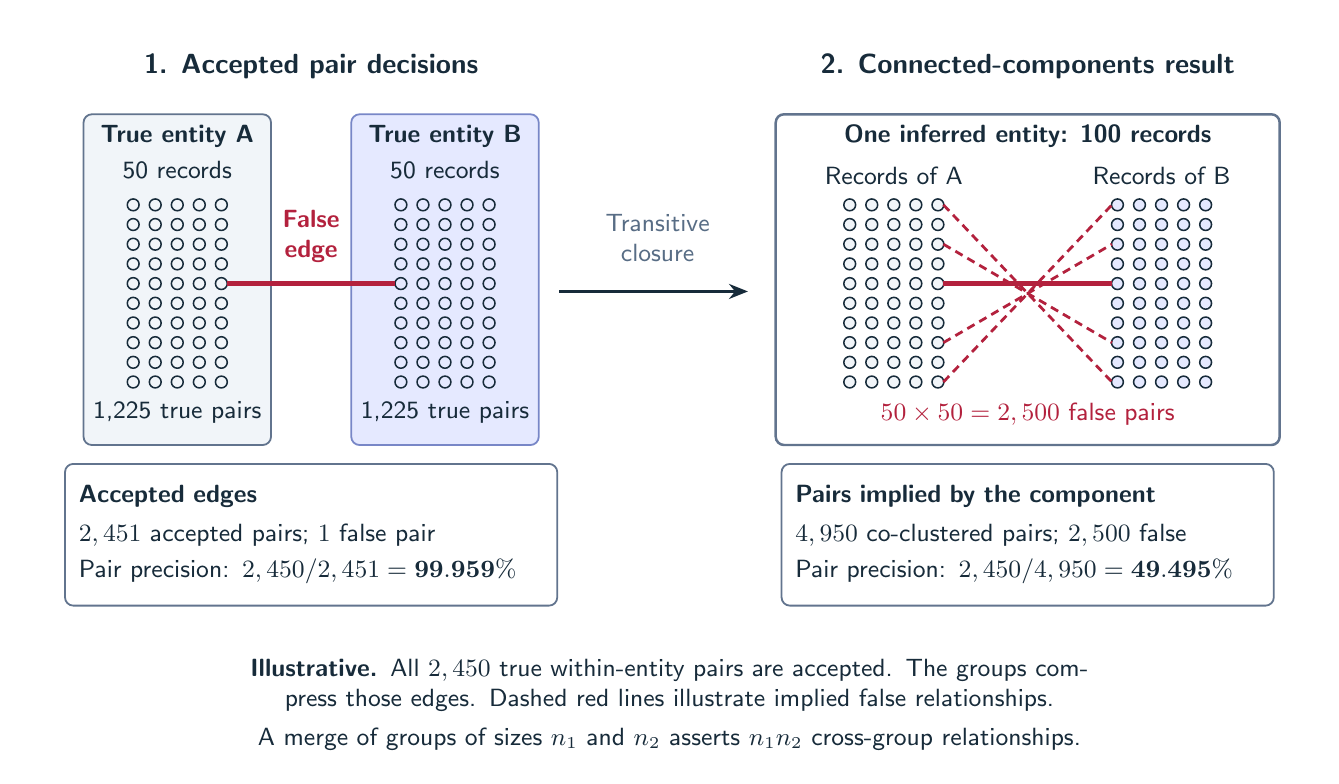
\begin{tikzpicture}[
  every node/.append style={font=\fontsize{9}{11}\selectfont},
  record/.style={circle,draw=ink,line width=.55pt,minimum size=1.5mm,inner sep=0pt},
  falseedge/.style={draw=errorink,line width=1.6pt},
  inferred/.style={draw=errorink,line width=1pt,dash pattern=on 3pt off 2pt},
]
\useasboundingbox (-.2,.3) rectangle (16.1,-8.95);

\node[font=\fontsize{10}{12}\selectfont\bfseries] at (3.4,-.2)
  {1. Accepted pair decisions};
\node[font=\fontsize{10}{12}\selectfont\bfseries] at (12.5,-.2)
  {2. Connected-components result};

\node[data,text width=21mm,minimum height=42mm,inner sep=4pt]
  (a) at (1.7,-2.9) {};
\node[model,text width=21mm,minimum height=42mm,inner sep=4pt]
  (b) at (5.1,-2.9) {};
\node[font=\fontsize{9}{11}\selectfont\bfseries] at (1.7,-1.08) {True entity A};
\node[font=\fontsize{9}{11}\selectfont\bfseries] at (5.1,-1.08) {True entity B};
\node at (1.7,-1.51) {50 records};
\node at (5.1,-1.51) {50 records};
\foreach \i in {0,...,4} {
  \foreach \j in {0,...,9} {
    \node[record,fill=datafill] at ({1.7+(.28*(\i-2))},{-1.95-.25*\j}) {};
    \node[record,fill=modelfill] at ({5.1+(.28*(\i-2))},{-1.95-.25*\j}) {};
  }
}
\draw[falseedge] (2.33,-2.95) -- (4.47,-2.95);
\node[text=errorink,text width=10mm,font=\fontsize{9}{11}\selectfont\bfseries]
  at (3.4,-2.35) {False\\edge};
\node at (1.7,-4.58) {1,225 true pairs};
\node at (5.1,-4.58) {1,225 true pairs};

\draw[flow] (6.55,-3.05) -- (9,-3.05);
\node[label,text width=18mm,font=\fontsize{9}{11}\selectfont]
  at (7.8,-2.37) {Transitive\\closure};

\draw[draw=dataline,fill=white,rounded corners=3pt,line width=.9pt]
  (9.3,-.8) rectangle (15.7,-5.0);
\node[font=\fontsize{9}{11}\selectfont\bfseries] at (12.5,-1.08)
  {One inferred entity: 100 records};
\node at (10.8,-1.58) {Records of A};
\node at (14.2,-1.58) {Records of B};
\foreach \i in {0,...,4} {
  \foreach \j in {0,...,9} {
    \node[record,fill=datafill] at ({10.8+(.28*(\i-2))},{-1.95-.25*\j}) {};
    \node[record,fill=modelfill] at ({14.2+(.28*(\i-2))},{-1.95-.25*\j}) {};
  }
}
\draw[falseedge] (11.43,-2.95) -- (13.57,-2.95);
\draw[inferred] (11.43,-1.95) -- (13.57,-4.20);
\draw[inferred] (11.43,-4.20) -- (13.57,-1.95);
\draw[inferred] (11.43,-2.45) -- (13.57,-3.70);
\draw[inferred] (11.43,-3.70) -- (13.57,-2.45);
\node[text=errorink] at (12.5,-4.61) {$50\times50 = 2,500$ false pairs};

\node[box,text width=59mm,minimum height=18mm,align=left]
  at (3.4,-6.14)
  {\textbf{Accepted edges}\\[3pt]
   $2,451$ accepted pairs; $1$ false pair\\[2pt]
   Pair precision: $2,450/2,451 = \mathbf{99.959\%}$};
\node[box,text width=59mm,minimum height=18mm,align=left]
  at (12.5,-6.14)
  {\textbf{Pairs implied by the component}\\[3pt]
   $4,950$ co-clustered pairs; $2,500$ false\\[2pt]
   Pair precision: $2,450/4,950 = \mathbf{49.495\%}$};

\node[text width=153mm,font=\fontsize{9}{11}\selectfont]
  at (7.95,-8.30)
  {\textbf{Illustrative.} All $2,450$ true within-entity pairs are accepted.
   The groups compress those edges. Dashed red lines illustrate implied false relationships.\\[3pt]
   A merge of groups of sizes $n_1$ and $n_2$ asserts $n_1n_2$ cross-group relationships.};
\end{tikzpicture}
\end{document}
